\documentclass[a4paper,12pt]{article} % тип документа

% report, book

% Рисунки
\usepackage{graphicx}
\usepackage{wrapfig}
\usepackage{mathtext}

\usepackage{hyperref}
\usepackage[rgb]{xcolor}
\hypersetup{				% Гиперссылки
    colorlinks=true,       	% false: ссылки в рамках
	urlcolor=blue          % на URL
}

%  Русский язык

\usepackage[T2A]{fontenc}			% кодировка
\usepackage[utf8]{inputenc}			% кодировка исходного текста
\usepackage[english,russian]{babel}	% локализация и переносы


% Математика
\usepackage{amsmath,amsfonts,amssymb,amsthm,mathtools} 


\usepackage{wasysym}

\author{Анна Назарчук Б02-109}
\title{2.1.3 Определение $c_p/c_v$ по скорости звука в газе}
\date{}
\begin{document}
\maketitle
\section{Аннотация}
Цель: 1) измерение частоты колебаний и длины волны при резонансе звуковых колебаний в газе, заполняющем трубу 
2) определение показателя адиабаты с помощью уравнения состояния идеального газа

Оборудование: звуковой генератор, электронный осциллограф, раздвижная труба, теплоизолированная труба, обогреваемая водой из термостата, баллон со сжатым углекислым газом, газгольдер.

\section{Теоретические сведения}
Скорость звука в газах определяется формулой:
\begin{equation}
c = \sqrt{\gamma \frac{RT}{\mu}}
\end{equation}
R - газовая постоянная, T -температура газа, $\mu$ - молярная масса, $\gamma$ - показатель адиабаты
Тогда:
\begin{equation}
\gamma = \frac{\mu}{RT}c^2
\end{equation} 
Условие резонанса (амплитуда звуковых колебаний резко возрастает):
\begin{equation}
L = n\frac{\lambda}{2}
\end{equation}
Связь параметров волны:
\begin{equation}
c=\lambda f
\end{equation}
Подбор условий резонанса:
1) f = const, $L\neq const$
\begin{equation}
L_{n+k} = n\frac{\lambda}{2} + k \frac{\lambda}{2}
\end{equation}
Тогда $\frac{\lambda}{2}$ - угловой коэффициент графика зависимости L от k.


2) L = const, $f\neq const$
\begin{equation}
L=\frac{\lambda_1}{2}n=\frac{\lambda_2}{2}(n+1)=...=\frac{\lambda_{k+1}}{2}(n+k)
\end{equation}
Тогда:
\begin{equation}
f_{k+1} = f_1+\frac{c}{2L}k
\end{equation}
Тогда $c/2L$ - угловой коэффициент графика зависимости частоты от номера резонанса.


\section{Экспериментальная установка}
В работе используются две установки (рис. \ref{схема1}, \ref{схема2}). Первая установка содержит раздвижную трубу с миллиметровой шкалой, наполняется газом из газгольдера. Производятся измерения для разных газов: воздуха и углекислого газа. Вторая установка содержит теплоизолированную трубу, которая нагревается водой из термостата. Измеряется зависимость скорости звука от температуры.

\begin{figure}[h!]
\begin{center}
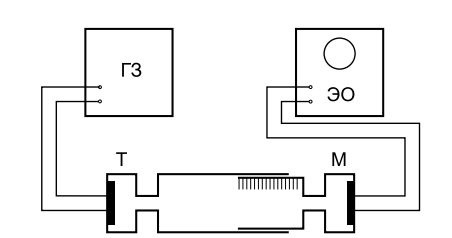
\includegraphics[width=0.9\textwidth]{Схема1.png}
\end{center}
\caption{Схема установки c раздвижной трубой} 
\label{схема1}
\end{figure}

\begin{figure}[h!]
\begin{center}
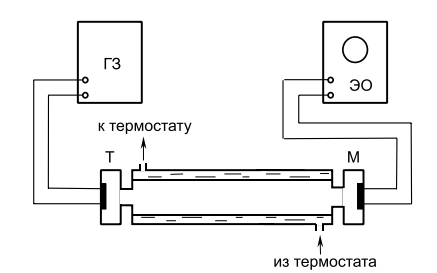
\includegraphics[width=0.9\textwidth]{Схема2}
\end{center}
\caption{Схема установки с термостатом} \label{схема2}
\end{figure} 

\section{Измерения и обработка данных}

\subsection{Измерения при постоянной длине трубы}
Данные измерений представлены в таблице \ref{tbl:температура} и на графике (рис. \ref{temperature}). Длина трубы $L = 740 \pm 1 мм$

\begin{table}[h!]
\caption{Зависимость частоты от номера резонанса при разных температурах для постоянной длины}
\label{tbl:температура}
\begin{tabular}{|ll|ll|ll|ll|ll|ll|}
\hline
\multicolumn{2}{|l|}{t = 22.4 $^\circ C$} & \multicolumn{2}{l|}{t = 30.1 $^\circ C$} & \multicolumn{2}{l|}{t = 40.2 $^\circ C$} & \multicolumn{2}{l|}{t = 50.1 $^\circ C$} & \multicolumn{2}{l|}{t = 55.1 $^\circ C$} & \multicolumn{2}{l|}{t = 60.1 $^\circ C$} \\ \hline
\multicolumn{1}{|l|}{k}      & f, Гц      & \multicolumn{1}{l|}{k}      & f, Гц      & \multicolumn{1}{l|}{k}     & f, Гц      & \multicolumn{1}{l|}{k}      & f, Гц      & \multicolumn{1}{l|}{k}      & f, Гц      & \multicolumn{1}{l|}{k}      & f, Гц      \\ \hline
\multicolumn{1}{|l|}{0}      & 251.4      & \multicolumn{1}{l|}{0}      & 256.5      & \multicolumn{1}{l|}{0}     & 257.8      & \multicolumn{1}{l|}{0}      & 260.4      & \multicolumn{1}{l|}{0}      & 263.9      & \multicolumn{1}{l|}{0}      & 264.1      \\ \hline
\multicolumn{1}{|l|}{1}      & 476.4      & \multicolumn{1}{l|}{1}      & 481.6      & \multicolumn{1}{l|}{1}     & 488.9      & \multicolumn{1}{l|}{1}      & 498.1      & \multicolumn{1}{l|}{1}      & 501.1      & \multicolumn{1}{l|}{1}      & 505.1      \\ \hline
\multicolumn{1}{|l|}{2}      & 703.1      & \multicolumn{1}{l|}{2}      & 711.9      & \multicolumn{1}{l|}{2}     & 722.7      & \multicolumn{1}{l|}{2}      & 734.5      & \multicolumn{1}{l|}{2}      & 739.7      & \multicolumn{1}{l|}{2}      & 745.3      \\ \hline
\multicolumn{1}{|l|}{3}      & 931.1      & \multicolumn{1}{l|}{3}      & 942.3      & \multicolumn{1}{l|}{3}     & 957.1      & \multicolumn{1}{l|}{3}      & 972.8      & \multicolumn{1}{l|}{3}      & 980.1      & \multicolumn{1}{l|}{3}      & 987.3      \\ \hline
\multicolumn{1}{|l|}{4}      & 1160.7     & \multicolumn{1}{l|}{4}      & 1174.9     & \multicolumn{1}{l|}{4}     & 1194.1     & \multicolumn{1}{l|}{4}      & 1212.3     & \multicolumn{1}{l|}{4}      & 1221.9     & \multicolumn{1}{l|}{4}      & 1230.7     \\ \hline
\multicolumn{1}{|l|}{}       &            & \multicolumn{1}{l|}{5}      & 1408.9     & \multicolumn{1}{l|}{5}     & 1435.7     & \multicolumn{1}{l|}{5}      & 1453.5     & \multicolumn{1}{l|}{5}      & 1464.2     & \multicolumn{1}{l|}{5}      & 1475.5     \\ \hline
\multicolumn{1}{|l|}{}       &            & \multicolumn{1}{l|}{6}      & 1641.9     & \multicolumn{1}{l|}{6}     & 1668.2     & \multicolumn{1}{l|}{6}      & 1694.1     & \multicolumn{1}{l|}{6}      & 1707.3     & \multicolumn{1}{l|}{}       &            \\ \hline
\multicolumn{1}{|l|}{}       &            & \multicolumn{1}{l|}{7}      & 1876.1     & \multicolumn{1}{l|}{}      &            & \multicolumn{1}{l|}{}       &            & \multicolumn{1}{l|}{}       &            & \multicolumn{1}{l|}{}       &            \\ \hline
\end{tabular}
\end{table}

\begin{figure}[h!]
\begin{center}
\includegraphics[width=0.9\textwidth]{temperature}
\end{center}
\caption{Зависимость частоты от номера резонанса для разных температур} \label{temperature}
\end{figure}

Коэффициент наклона графика - $c/2L$. Для каждой температуры посчитаем скорость звука и представим в таблице \ref{tbl:c_T} и на графике \ref{img:c_T}
\begin{table}[h!] 
 \caption{Зависимость скорости звука от температуры}
\label{tbl:c_T}
  \begin{tabular}{|c|c|c|} \hline c, м/с & $\sigma_c$, м/с  & T, K \\ \hline 336.448 & 0.884 & 295.4 \\ \hline 342.907 & 0.914 & 303.1 \\ \hline 348.656 & 1.033 & 313.2 \\ \hline 353.598 & 0.75 & 323.1 \\ \hline 356.183 & 0.85 & 328.1 \\ \hline 358.405 & 0.798 & 333.1 \\ \hline
\end{tabular} 
\end{table}

\begin{figure}[h!]
\begin{center}
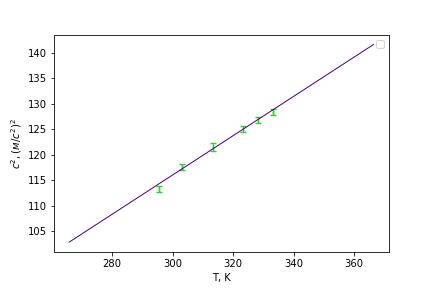
\includegraphics[width=0.9\textwidth]{CC_T}
\end{center}
\caption{Зависимость квадрата скорости звука от температуры} \label{img:c_T}
\end{figure}

Из коэффициента наклона графика и формулы:
\begin{equation}
\gamma = \frac{\mu}{RT}c^2
\end{equation}
Найдем значение для показателя адиабаты в воздухе:
$\gamma = 1.35 \pm 0.01$


\subsection{Измерения при постоянной температуре для воздуха}
Данные измерений представлены в таблице \ref{tbl:воздух} и на графике (рис. \ref{частота_air}). Температура $T = 293 K$.

\begin{table}[h!]
\caption{Зависимость длины трубы от номера резонанса при разных частотах для постоянной температуры для воздуха}
\label{tbl:воздух}
\begin{tabular}{|ll|ll|ll|ll|ll|}
\hline
\multicolumn{2}{|l|}{f = 4412 Гц} & \multicolumn{2}{l|}{f = 3707 Гц} & \multicolumn{2}{l|}{f = 3011 Гц} & \multicolumn{2}{l|}{f = 5092 Гц} & \multicolumn{2}{l|}{f = 5406 Гц} \\ \hline
\multicolumn{1}{|l|}{k}  & L, мм  & \multicolumn{1}{l|}{k}  & L, мм  & \multicolumn{1}{l|}{k}  & L, мм  & \multicolumn{1}{l|}{k}  & L, мм  & \multicolumn{1}{l|}{k}  & L, мм  \\ \hline
\multicolumn{1}{|l|}{0}  & 20     & \multicolumn{1}{l|}{0}  & 36     & \multicolumn{1}{l|}{0}  & 58     & \multicolumn{1}{l|}{0}  & 8      & \multicolumn{1}{l|}{0}  & 35     \\ \hline
\multicolumn{1}{|l|}{1}  & 55     & \multicolumn{1}{l|}{1}  & 87     & \multicolumn{1}{l|}{1}  & 115    & \multicolumn{1}{l|}{1}  & 41     & \multicolumn{1}{l|}{1}  & 99     \\ \hline
\multicolumn{1}{|l|}{2}  & 96     & \multicolumn{1}{l|}{2}  & 129    & \multicolumn{1}{l|}{2}  & 172    & \multicolumn{1}{l|}{2}  & 76     & \multicolumn{1}{l|}{2}  & 133    \\ \hline
\multicolumn{1}{|l|}{3}  & 131    & \multicolumn{1}{l|}{3}  & 180    & \multicolumn{1}{l|}{3}  & 229    & \multicolumn{1}{l|}{3}  & 109    & \multicolumn{1}{l|}{3}  & 160    \\ \hline
\multicolumn{1}{|l|}{4}  & 172    & \multicolumn{1}{l|}{4}  & 220    & \multicolumn{1}{l|}{}   &        & \multicolumn{1}{l|}{4}  & 143    & \multicolumn{1}{l|}{4}  & 197    \\ \hline
\end{tabular}
\end{table}

\begin{figure}[h!]
\begin{center}
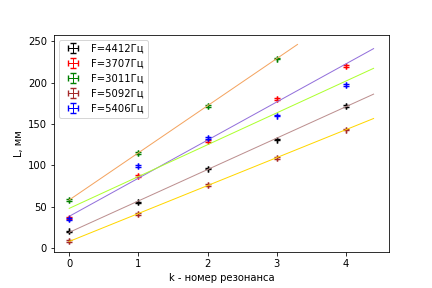
\includegraphics[width=0.9\textwidth]{Frequency_air}
\end{center}
\caption{Зависимость длины трубы от номера резонанса для воздуха} \label{частота_air}
\end{figure}

Угловой коэффициент - $\lambda/2$. Найдем длину волны для каждой частоты, результаты в таблице \ref{tbl:lambda_f} и на графике \ref{img:lambda_f}.

\begin{table}[h!] \caption{Зависимость длины волны от частоты для воздуха} \label{tbl:lambda_f} \begin{tabular}{|c|c|c|} \hline $\lambda$, мм & $f$, Гц & $\sigma_\lambda$, мм \\ \hline 76.0 & 4412 & 1.443 \\ \hline 92.2 & 3707 & 2.217 \\ \hline 114.0 & 3011 & 0.794 \\ \hline 67.6 & 5092 & 0.954 \\ \hline 77.0 & 5406 & 7.564 \\ \hline \end{tabular} \end{table}

\begin{figure}[h!]
\begin{center}
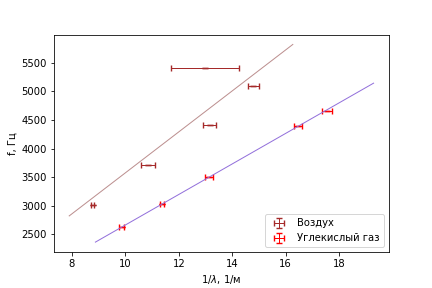
\includegraphics[width=0.9\textwidth]{f(la)}
\end{center}
\caption{Зависимость частоты от обратного к длине волны для воздуха и углексилого газа при постоянной температуре} \label{img:lambda_f}
\end{figure}

Тогда скорость звука - угловой коэффициент на графике. ($c= 357.8 \pm 15.8 м/с$)В таком случае из него и формулы:
\begin{equation}
\gamma = \frac{\mu}{RT}c^2
\end{equation}
Найдем значение для показателя адиабаты в воздухе:
$\gamma = 1.53 \pm 0.2$
Погрешность столь велика из-за неточного поиска длин трубы, при которых происходит резонанс.

\subsection{Измерения при постоянной температуре для углекислого газа}
Данные измерений представлены в таблице \ref{tbl:углекислый газ} и на графике (рис. \ref{частота_co2}). Температура $T = 293 K$.

\begin{table}[h!]
\caption{Зависимость длины трубы от номера резонанса при разных частотах для постоянной температуры для углекислого газа}
\label{tbl:углекислый газ}
\begin{tabular}{|ll|ll|ll|ll|ll|}
\hline
\multicolumn{2}{|l|}{f = 4398 Гц} & \multicolumn{2}{l|}{f = 4665 Гц} & \multicolumn{2}{l|}{f = 3506 Гц} & \multicolumn{2}{l|}{f = 3039 Гц} & \multicolumn{2}{l|}{f = 2624Гц} \\ \hline
\multicolumn{1}{|l|}{k}  & L, мм  & \multicolumn{1}{l|}{k}  & L, мм  & \multicolumn{1}{l|}{k}  & L, мм  & \multicolumn{1}{l|}{k}  & L, мм  & \multicolumn{1}{l|}{k}  & L, мм \\ \hline
\multicolumn{1}{|l|}{0}  & 52     & \multicolumn{1}{l|}{0}  & 99     & \multicolumn{1}{l|}{0}  & 47     & \multicolumn{1}{l|}{0}  & 50     & \multicolumn{1}{l|}{0}  & 45    \\ \hline
\multicolumn{1}{|l|}{1}  & 81     & \multicolumn{1}{l|}{1}  & 127    & \multicolumn{1}{l|}{1}  & 86     & \multicolumn{1}{l|}{1}  & 94     & \multicolumn{1}{l|}{1}  & 95    \\ \hline
\multicolumn{1}{|l|}{2}  & 112    & \multicolumn{1}{l|}{2}  & 157    & \multicolumn{1}{l|}{2}  & 124    & \multicolumn{1}{l|}{2}  & 138    & \multicolumn{1}{l|}{2}  & 146   \\ \hline
\multicolumn{1}{|l|}{3}  & 143    & \multicolumn{1}{l|}{3}  & 184    & \multicolumn{1}{l|}{3}  & 163    & \multicolumn{1}{l|}{3}  & 182    & \multicolumn{1}{l|}{3}  & 197   \\ \hline
\multicolumn{1}{|l|}{4}  & 173    & \multicolumn{1}{l|}{4}  & 213    & \multicolumn{1}{l|}{}   & 199    & \multicolumn{1}{l|}{4}  & 226    & \multicolumn{1}{l|}{}   &       \\ \hline
\multicolumn{1}{|l|}{5}  & 203    & \multicolumn{1}{l|}{}   &        & \multicolumn{1}{l|}{}   &        & \multicolumn{1}{l|}{}   &        & \multicolumn{1}{l|}{}   &       \\ \hline
\end{tabular}
\end{table}

\begin{figure}[h!]
\begin{center}
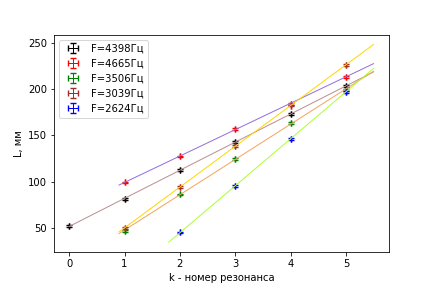
\includegraphics[width=0.9\textwidth]{Frequency_co2}
\end{center}
\caption{Зависимость длины трубы от номера резонанса для углекислого газа} \label{частота_co2}
\end{figure} 

Угловой коэффициент - $\lambda/2$. Найдем длину волны для каждой частоты, результаты в таблице \ref{tbl:lambda_f_co2} и на графике \ref{img:lambda_f}.

\begin{table}[h!] \caption{Зависимость длины волны от частоты для углекислого газа} \label{tbl:lambda_f_co2} \begin{tabular}{|c|c|c|} \hline $\lambda$, мм & $f$, Гц & $\sigma_\lambda$, мм \\ \hline 60.686 & 4398 & 0.548 \\ \hline 57.0 & 4665 & 0.577 \\ \hline 76.2 & 3506 & 0.86 \\ \hline 88.0 & 3039 & 0.638 \\ \hline 101.4 & 2624 & 0.908 \\ \hline \end{tabular} \end{table}

Тогда скорость звука - угловой коэффициент на графике. ($c= 266.6 \pm 0.3 м/с$)В таком случае из него и формулы:
\begin{equation}
\gamma = \frac{\mu}{RT}c^2
\end{equation}
Найдем значение для показателя адиабаты в углекислом газе:
$\gamma = 1.29 \pm 0.01$

\section{Вывод}

\hspace{5mm}
1. Получена зависимость скорости звука в газе от температуры, полученная корень-зависимость совпадает с теоретическим расчетом.

2. Получены значения показателя адиабаты для воздуха: $\gamma_1 = 1.53 \pm 0.2$, $\gamma_2 = 1.35 \pm 0.01$ (для изменения длины трубы и частоты соответственно). Теоретическое значение $\gamma = 1.4$, что лежит в погрешности полученных значений.

3. Получено значение показателя адиабаты для углекислого газа: $\gamma =  1.29 \pm 0.01$. Теоретическое значение  $\gamma = 1.3$, что схоже с полученным результатом.

\end{document}